\section{Nutrition}

\begin{multicols}{2}


%\section*{Human Nutrition}

%==================================================================================================%

\section*{Properties of Food Substances}


\subsection{Lipids - Fats and Oils} % VSO 26

\begin{center}
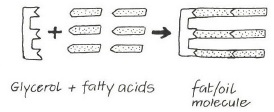
\includegraphics[width=0.4\textwidth]{./img/vso/lipids.jpg}
\end{center}

\begin{description*}
%\item[Subtopic:]{}
\item[Materials:]{Card, scissors}
\item[Setup:]{Cut out the shapes of the glycerol and fatty acid molecules. They can be
combined to form fat (lipid) molecules.}
\item[Procedure:]{Ask students to form fats of different types with the cards. }
%\item[Hazards:]{}
%\item[Questions:]{}
%\item[Observations:]{}
\item[Theory:]{Fats are made up of glycerol and fatty acids. The longer the fatty acid chains
the more solid the lipid. Oils have short chains of fatty acids, fats much
longer ones.}
%\item[Applications:]{}
%\item[Notes:]{}
\end{description*}

\subsection{Solubility of Fats and Oils} % Source 41

\begin{center}
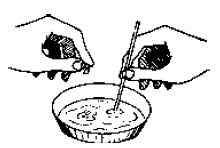
\includegraphics[width=0.4\textwidth]{./img/source/fats-oils-solubility.png}
\end{center}

\begin{description*}
%\item[Subtopic:]{}
\item[Materials:]{Oil, water, petrol, 2 containers}
%\item[Setup:]{}
\item[Procedure:]{Mix fats or oil with water. Then in a separate container mix fats or oils with a small amount
of petrol.}
%\item[Hazards:]{}
\item[Questions:]{Look through the two liquids. Is there a difference?}
\item[Observations:]{Oils and fats dissolve in organic solvents such as petrol or alcohol, but not in water.
However, vigorous shaking with water will produce a cloudy or milky emulsion of suspended
fat droplets.}
%\item[Theory:]{}
%\item[Applications:]{}
%\item[Notes:]{}
\end{description*}

\subsection{Carbohydrates} % VSO 26

\begin{center}
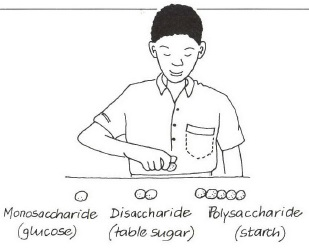
\includegraphics[width=0.4\textwidth]{./img/vso/carbohydrates.jpg}
\end{center}

\begin{description*}
%\item[Subtopic:]{}
\item[Materials:]{Peas, beans or other small identical items}
%\item[Setup:]{}
\item[Procedure:]{Arrange peas or other small objects to make carbohydrate chains of different lengths.}
%\item[Hazards:]{}
%\item[Questions:]{}
%\item[Observations:]{}
\item[Theory:]{Each pea is a monosaccharide,
e.g. glucose. Putting 2 together
makes a disaccharide, e.g. table
sugar, and a long chain of them a
polysaccharide, e.g. starch. 
}
%\item[Applications:]{Toilet
%roll provides another analogy of
%the way identical units combine in
%long chains to make a polysaccharide.}
\item[Notes:]{Not all di- and
polysaccharides consist of
identical units, e.g. sucrose is a
disaccharide of 2 monosaccharides
glucose and fructose.}
\end{description*}

\subsection{Simple Sugar Model} % Source 39

\begin{center}
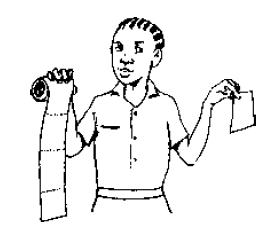
\includegraphics[width=0.4\textwidth]{./img/source/sugar-model.png}
\end{center}

\begin{description*}
%\item[Subtopic:]{}
%\item[Materials:]{}
%\item[Setup:]{}
\item[Procedure:]{To illustrate the long chain structure of polysaccharides use strings of beads, toilet roll or a
chain of pupils. Each long chain is formed by smaller units which represent simple sugars.}
%\item[Hazards:]{}
%\item[Questions:]{}
%\item[Observations:]{}
%\item[Theory:]{}
%\item[Applications:]{}
%\item[Notes:]{}
\end{description*}

\subsection{Protein Molecules} % VSO 26

\begin{center}
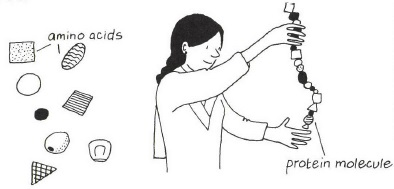
\includegraphics[width=0.45\textwidth]{./img/vso/proteins.jpg}
\end{center}

\begin{description*}
%\item[Subtopic:]{}
\item[Materials:]{Bottle caps, seeds, beans, fruits, paper/card, string, scissors}
%\item[Setup:]{}
\item[Procedure:]{A variety of different shaped and
sized items threaded on a string
show how different types of
amino acids join together to
make a protein molecule.
Students can collect their own
materials and make their own
models, or cut out
shapes from paper or card.}
%\item[Hazards:]{}
%\item[Questions:]{}
%\item[Observations:]{}
%\item[Theory:]{}
%\item[Applications:]{}
%\item[Notes:]{}
\end{description*}

\subsection{Straightening Hair} % Source 44

\begin{center}
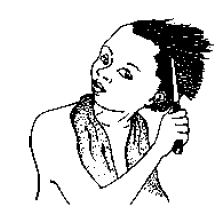
\includegraphics[width=0.35\textwidth]{./img/source/straight-hair.png}
\end{center}

\begin{description*}
%\item[Subtopic:]{}
%\item[Materials:]{}
%\item[Setup:]{}
%\item[Procedure:]{}
%\item[Hazards:]{}
\item[Observations:]{Some Tanzanian women use a hot comb to straighten their hair.}
\item[Questions:]{Why can't a cold comb be used?}
\item[Theory:]{The protein keratin, which is present in hair, has sulphur bonds between protein chains.
Combing the hair with a hot comb can break these bonds temporarily and thus straighten the
hair. The bonds soon rejoin and the hair becomes kinky again.}
%\item[Applications:]{}
%\item[Notes:]{}
\end{description*}

%==================================================================================================%

\section*{Food Tests}
%\textbf{*NECTA PRACTICAL*}


\subsection{Test for Lipids} % VSO 27, LASM 70

\begin{center}
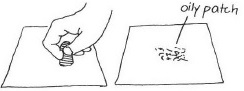
\includegraphics[width=0.4\textwidth]{./img/vso/food-test-lipids.jpg}
\end{center}

\begin{description*}
%\item[Subtopic:]{}
\item[Materials:]{Cooking oil, water, plastic bottles, \nameref{sec:testtubes}*, iodine solution, straw}
%\item[Setup:]{}
\item[Procedure:]{Mix about 10 mL of cookingoil and about 100 mL of water in a plastic bottle and shake vigorously. Pour a small amount into a test tube or syringe. Add 3 drops of iodine solution using a straw and shake the tube.}
%\item[Hazards:]{}
%\item[Questions:]{}
\item[Observations:]{You should see the formation of a red ring at the top of the solution, indicating the presence of lipids.}
%\item[Theory:]{}
%\item[Applications:]{}
\item[Notes:]{Alternatively, rub a piece of food onto a piece of paper. Fat is present if there is a translucent stain.}
\end{description*}

\subsection{Test for Protein} % VSO 27

\begin{center}
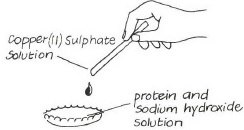
\includegraphics[width=0.4\textwidth]{./img/vso/food-test-protein.jpg}
\end{center}

\begin{description*}
%\item[Subtopic:]{}
\item[Materials:]{Copper (II) sulphate solution*, sodium hydroxide solution*, food sample (e.g. egg), bottle cap, straw}
%\item[Setup:]{}
\item[Procedure:]{Pour a small amount of egg white into a bottle cap. Add a few drops of sodium hydroxide solution, followed by a small amount of copper (II) sulphate solution.}
%\item[Hazards:]{}
%\item[Questions:]{}
\item[Observations:]{Purple colour indicates the presence of protein in the sample.}
%\item[Theory:]{}
%\item[Applications:]{}
%\item[Notes:]{}
\end{description*}

\subsection{Test for Starch} % VSO 27

\begin{center}
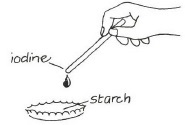
\includegraphics[width=0.4\textwidth]{./img/vso/food-test-starch.jpg}
\end{center}

\begin{description*}
%\item[Subtopic:]{}
\item[Materials:]{Maize flour, iodine solution, bottle cap, water, straw}
\item[Setup:]{Prepare a food sample solution by either saving the remaining water from boiling pasta/potatoes or by mixing 2 teaspoons of maize flour into a litre of water and heating to dissolve.}
\item[Procedure:]{Add a few drops of iodine solution to the sample and observe any changes.}
%\item[Hazards:]{}
%\item[Questions:]{}
\item[Observations:]{A blue-black colour confirms the presence of starch.}
%\item[Theory:]{}
%\item[Applications:]{}
%\item[Notes:]{}
\end{description*}

\subsection{Test for Reducing Sugars} % VSO 27

\begin{center}
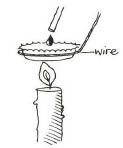
\includegraphics[width=0.25\textwidth]{./img/vso/food-test-reducing.jpg}
\end{center}

\begin{description*}
%\item[Subtopic:]{}
\item[Materials:]{Benedict's solution*, \nameref{sec:heatsources}*, bottle cap, straw, food sample (e.g. glucose or onions)}
%\item[Setup:]{}
\item[Procedure:]{Dissolve the food in water. Put
some into the bottle top and add
Benedict's solution.
Heat very gently for 1 minute.}
\item[Hazards:]{Safety goggles should be worn. }
%\item[Questions:]{}
\item[Observations:]{If
a precipitate develops - usually
green or brown - this confirms
the presence of sugar.}
%\item[Theory:]{}
%\item[Applications:]{}
%\item[Notes:]{}
\end{description*}

\subsection{Test for Non-Reducing Sugars}

%\begin{center}
%\includegraphics[width=0.4\textwidth]{./img/.png}
%\end{center}

\begin{description*}
%\item[Subtopic:]{}
\item[Materials:]{Benedict's solution*, \nameref{sec:heatsources}*, sodium hydroxide solution*, citric acid, water, food sample (e.g. sugar/sugar cane), }
%\item[Setup:]{}
\item[Procedure:]{Prepare a food sample solution by adding water. Add a small amount of citric acid to the solution and bring to a boil. Allow it to cool and add a small amount of NaOH to the solution and shake. Add a small amount of Benedict's solution and boil again. Allow it to cool and observe changes in appearance.}
%\item[Hazards:]{}
%\item[Questions:]{}
\item[Observations:]{A colour change from green to yellow, then to brick red precipitate indicates the presence of non-reducing sugars.}
%\item[Theory:]{}
%\item[Applications:]{}
%\item[Notes:]{}
\end{description*}

%==================================================================================================%

\section*{Human Digestive System}


\subsection{Models for Digestion} % VSO 27

\begin{center}
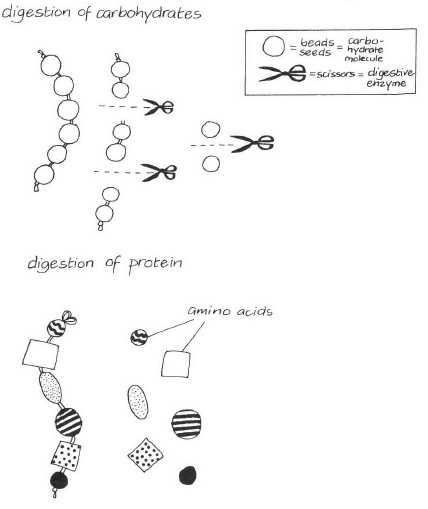
\includegraphics[width=0.49\textwidth]{./img/vso/digestion-models.jpg}
\end{center}

\begin{description*}
%\item[Subtopic:]{}
\item[Materials:]{Beads/seeds/cards, scissors, string}
%\item[Setup:]{}
\item[Procedure:]{String several beads or seeds together to make a chain. Or use toiler paper sheets or paper clips. Cut up or separate the models of food molecules to
demonstrate digestion.}
%\item[Hazards:]{}
\item[Questions:]{What action does cutting with scissors represent?}
\item[Observations:]{The scissor action represents the action of salivary amylase as it breaks down the long
starch chain to simple sugars (maltose).}
\item[Theory:]{Starch is a polysaccharide made up of many identical glucose molecules. 27
Proteins are made up from many different amino acids. During
digestion large molecules are broken down into smaller ones by
enzymes, e.g. starch is broken down into glucose, proteins into the
component amino acids.}
%\item[Applications:]{}
%\item[Notes:]{}
\end{description*}

\subsection{Digestive System Model} % VSO 28

\begin{center}
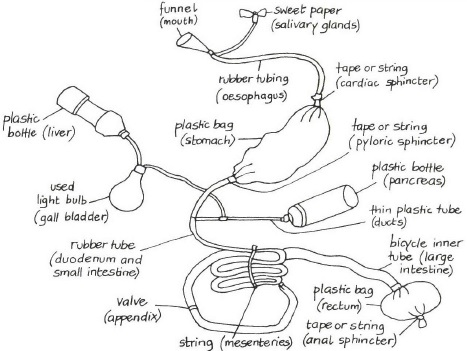
\includegraphics[width=0.49\textwidth]{./img/vso/digestive-sys-model.jpg} \\[6pt]
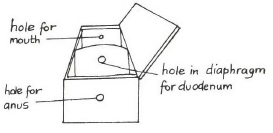
\includegraphics[width=0.4\textwidth]{./img/vso/digestive-sys-model-2.jpg}
\end{center}

\begin{description*}
%\item[Subtopic:]{}
%\item[Materials:]{}
%\item[Setup:]{}
\item[Procedure:]{Have students construct a model of a digestive system using the local materials shown. Colour and label the different sections and mount on a display board. }
%\item[Hazards:]{}
%\item[Questions:]{}
%\item[Observations:]{}
%\item[Theory:]{}
\item[Applications:]{Ask students to place inside a box to demonstrate how the intestine passes through the diaphragm.}
%\item[Notes:]{}
\end{description*}

\subsection{Types of Teeth} % Source 53

\begin{center}
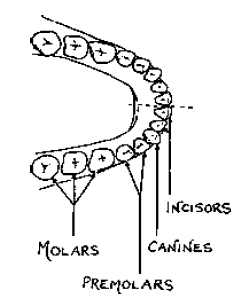
\includegraphics[width=0.3\textwidth]{./img/source/teeth-types.png}
\end{center}

\begin{description*}
%\item[Subtopic:]{}
%\item[Materials:]{}
%\item[Setup:]{}
\item[Procedure:]{Look into a friend's mouth. Examine the teeth and differentiate between them. Count the
number of each type present. Try to identify the function of each.}
%\item[Hazards:]{}
\item[Questions:]{How many are there altogether of each type?}
\item[Observations:]{There are four types of teeth in the buccal cavity and 32 teeth in all.}
\item[Theory:]{The four different types of teeth perform different functions. The front ones, the incisors,
are used for cutting. The canines are used for tearing. The premolars may have one or more
points for cutting, or flat surfaces for grinding. Behind the premolars are the molars with flat
surfaces for grinding. Molars are not present in young children.}
%\item[Applications:]{}
%\item[Notes:]{}
\end{description*}

\subsection{Invisible Saliva Ink} % VSO 29, Source 61

\begin{center}
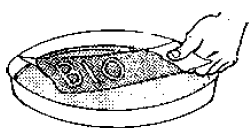
\includegraphics[width=0.4\textwidth]{./img/source/saliva-ink.png}
\end{center}

\begin{description*}
%\item[Subtopic:]{}
\item[Materials:]{Filter paper/toilet paper, starch solution, iodine solution, matches/cotton swabs}
\item[Setup:]{Prepare a starch solution by adding a teaspoon of maize/cassava flour to half a
cup of water. Bring to a boil, then allow to cool and filter the liquid through a cloth.}
\item[Procedure:]{Soak toilet paper in starch solution. Ask students to use saliva on a matchstick or cotton swab to write their names on the treated paper. Dip the paper in a very dilute iodine solution.}
%\item[Hazards:]{}
%\item[Questions:]{}
%\item[Observations:]{}
\item[Theory:]{The enzymes in the saliva digest the starch where it touches the paper.}
%\item[Applications:]{Enzyme action}
%\item[Notes:]{}
\end{description*}

\subsection{Salts in Saliva} % Source 62

\begin{center}
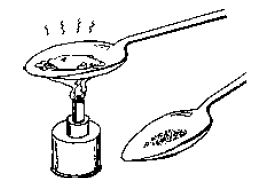
\includegraphics[width=0.4\textwidth]{./img/source/saliva-salts.png}
\end{center}

\begin{description*}
%\item[Subtopic:]{}
\item[Materials:]{Spoon, candle, dilute HCl}
%\item[Setup:]{}
\item[Procedure:]{Gently heat some saliva on a spoon until it is dry and observe. Then add a small amount of dilute hydrochloric acid.}
%\item[Hazards:]{}
%\item[Questions:]{}
\item[Observations:]{A white residue is left upon heating. Bubbles of carbon dioxide are given off when HCl is added.}
\item[Theory:]{Calcium carbonate is the residue and this reacts with the hydrochloric acid to produce
carbon dioxide.}
%\item[Applications:]{}
%\item[Notes:]{}
\end{description*}

\subsection{Swallowing Upside Down} % Shika 220, Source 64

\begin{center}
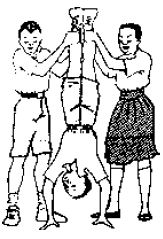
\includegraphics[width=0.35\textwidth]{./img/source/peristalsis.png}
\end{center}

\begin{description*}
%\item[Subtopic:]{}
\item[Materials:]{Drinking water/bread}
%\item[Setup:]{}
\item[Procedure:]{Drink a mouth full of water from a cup and swallow it. Then fill your mouth again, (without
swallowing) and with the help of two friends do a handstand. Then swallow while upside down. Also try with a small piece of bread}
%\item[Hazards:]{}
%\item[Questions:]{}
\item[Observations:]{You are able to swallow while upside down, but not as easily.}
\item[Theory:]{The peristalsis of the
esophagus works against the forces of gravity.}
%\item[Applications:]{}
%\item[Notes:]{}
\end{description*}

\subsection{Peristalsis Model} % VSO 29

\begin{center}
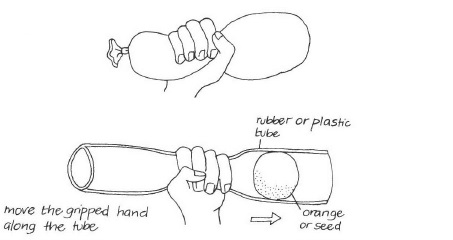
\includegraphics[width=0.49\textwidth]{./img/vso/peristalsis-model.jpg}
\end{center}

\begin{description*}
%\item[Subtopic:]{}
\item[Materials:]{Balloon, rubber band, orange/large seed, large tube}
%\item[Setup:]{}
\item[Procedure:]{A balloon gripped with the hand
pushes air along. You can also
move an object along a tube by
squeezing behind the `food' ball.}
%\item[Hazards:]{}
%\item[Questions:]{}
%\item[Observations:]{}
\item[Theory:]{Food is moved by the contraction
of the muscular walls of the gut.}
%\item[Applications:]{}
%\item[Notes:]{}
\end{description*}

\subsection{Intestine Length} % VSO 28, Source 71

\begin{center}
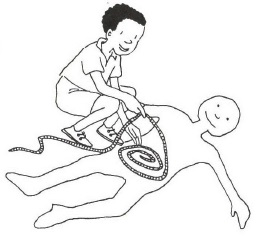
\includegraphics[width=0.4\textwidth]{./img/vso/intestine-length.jpg}
\end{center}

\begin{description*}
%\item[Subtopic:]{}
\item[Materials:]{Long piece of rope}
%\item[Setup:]{}
\item[Procedure:]{Ask pupils to draw on the ground the shapes of different animals (e.g. rabbit, man, cat/dog,
pig, cow). Try to draw them life size. Then coil string or strips of paper inside the abdominal
cavity area of the animal shape. Approximate lengths of intestines: rabbit 1~m
cat/dog 2~-~5~m, pig 24~m, horse 30~m, cow 50~m.}
%\item[Hazards:]{}
\item[Questions:]{Why do intestine lengths differ an why do herbivores have longer intestines than carnivores?}
%\item[Observations:]{}
\item[Theory:]{Length of intestine corresponds to the type of diet an animal eats. Herbivores have longer
intestines than carnivores in order to break down the plants that they eat.}
%\item[Applications:]{}
%\item[Notes:]{}
\end{description*}

\subsection{Absorption Model} % VSO 29

\begin{center}
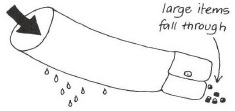
\includegraphics[width=0.4\textwidth]{./img/vso/absorption-model.jpg}
\end{center}

\begin{description*}
%\item[Subtopic:]{}
\item[Materials:]{Old shirt sleeve, small objects (e.g. peas), water}
%\item[Setup:]{}
\item[Procedure:]{Place the shirt sleeve over a container to catch the water as it drips
through. Pour the mixture of water and peas down the tube. }
%\item[Hazards:]{}
%\item[Questions:]{}
\item[Observations:]{Water
will leak out, but the peas (undigested food) pass straight down. You
may need to tie off the end of the sleeve to slow the process down.}
%\item[Theory:]{}
%\item[Applications:]{}
\item[Notes:]{Extend the activity by using a semi-permeable plastic bag for the gut.
Pour starch and sugar into the tube and test to see what passed
through.}
\end{description*}

%==================================================================================================%

\section*{Disorders of the Digestive System}


\subsection{Tooth Decay from Soda} % eggs in soda

\begin{center}
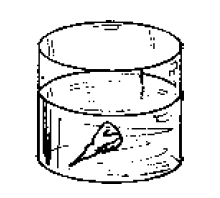
\includegraphics[width=0.35\textwidth]{./img/source/tooth-decay.png}
\end{center}

\begin{description*}
%\item[Subtopic:]{}
\item[Materials:]{Soda, glass, egg or baby tooth}
%\item[Setup:]{}
\item[Procedure:]{Place an egg or old baby tooth into a glass of soda (e.g. coke) and let it sit. Place another egg or tooth in water for comparison. After a while remove the eggs and observe.}
%\item[Hazards:]{}
%\item[Questions:]{}
\item[Observations:]{The soda has reacted with the egg shell or tooth enamel, digesting part of it.}
\item[Theory:]{When a person fails to brush their teeth properly, the food that remains on the teeth is acted
upon by the bacteria producing acids. These acids eat away the enamel and dentine causing
tooth decay.}
%\item[Applications:]{}
\item[Notes:]{Try with dilute HCl in place of soda.}
\end{description*}

%\subsection{Indigestion} % Source 67
%
%\begin{center}
%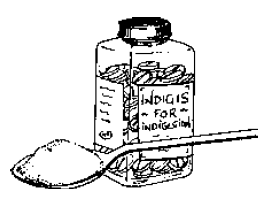
\includegraphics[width=0.4\textwidth]{./img/source/indigestion.png} % Source 67
%\end{center}
%
%\begin{description*}
%%\item[Subtopic:]{}
%\item[Materials:]{}
%\item[Setup:]{}
%\item[Procedure:]{}
%\item[Hazards:]{}
%\item[Questions:]{}
%\item[Observations:]{}
%\item[Theory:]{}
%\item[Applications:]{}
%\item[Notes:]{}
%\end{description*}

%==================================================================================================%

\section*{Nutrition in Plants}


\subsection{Nutrients from Soil} % Source 76

\begin{center}
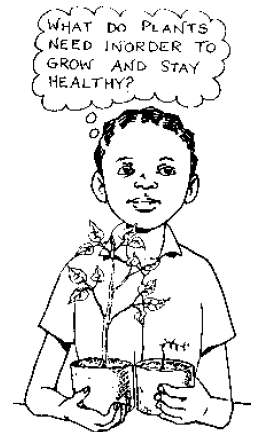
\includegraphics[width=0.3\textwidth]{./img/source/nutrients-plants.png}
\end{center}

\begin{description*}
%\item[Subtopic:]{}
\item[Materials:]{2 containers, cardboard, soil, seeds}
%\item[Setup:]{}
\item[Procedure:]{Fill one container with pieces of card board or foam packing cut
into very small pieces. Fill another container with fertile soil and plant a few seeds (peas,
beans or maize) in each one. Water each container throughout the experiment. Examine daily.}
%\item[Hazards:]{}
%\item[Questions:]{}
\item[Observations:]{Seedlings grown in the container without soil are smaller and less healthy with yellow leaves.}
\item[Theory:]{As well as water, carbon dioxide and sunlight, plants require mineral salts in order to grow
and remain healthy. The seedlings grown without soil get only water and so are lacking these
salts.}
%\item[Applications:]{}
%\item[Notes:]{}
\end{description*}

\subsection{Photosynthesis Model} % VSO 38

\begin{center}
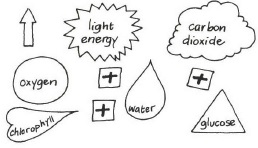
\includegraphics[width=0.45\textwidth]{./img/vso/photo-model.jpg}
\end{center}

\begin{description*}
%\item[Subtopic:]{}
\item[Materials:]{Card/paper, matches}
%\item[Setup:]{}
\item[Procedure:]{Draw and cut out the symbols shown above. Then arrange them in the correct order to
show the chemical equation for photosynthesis. Use matchsticks for arrows and + symbols.}
%\item[Hazards:]{}
%\item[Questions:]{}
%\item[Observations:]{}
%\item[Theory:]{}
%\item[Applications:]{}
\item[Notes:]{Repeat the above procedure but replace the words in the shapes with the chemical
formulae of the substances involved. These may be written on the reverse side of the first set
of cards.}
\end{description*}

\subsection{Photosynthesis Equation Game} % VSO 39

\begin{center}
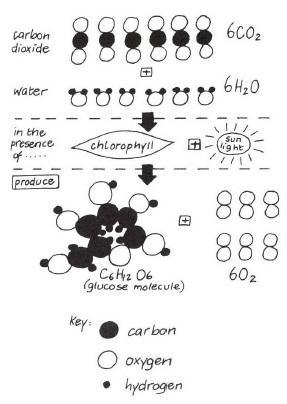
\includegraphics[width=0.45\textwidth]{./img/vso/photo-game.jpg}
\end{center}

\begin{description*}
%\item[Subtopic:]{}
\item[Materials:]{Beans, stones, coins, bottle caps, etc.}
%\item[Setup:]{}
\item[Procedure:]{Arrange the items so they
represent the stages of
photosynthesis as shown in the
diagram.}
%\item[Hazards:]{}
%\item[Questions:]{}
%\item[Observations:]{}
%\item[Theory:]{}
%\item[Applications:]{}
%\item[Notes:]{}
\end{description*}

\subsection{Leaf Structure} % LASM 81 / Leaf Sketch Shika 239

\begin{center}
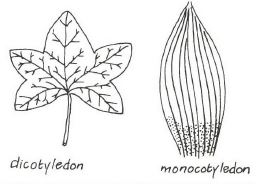
\includegraphics[width=0.4\textwidth]{./img/vso/leaf-structure.jpg}
\end{center}

\begin{description*}
%\item[Subtopic:]{}
\item[Materials:]{White paper, leaves, pencils}
%\item[Setup:]{}
\item[Procedure:]{Cover a leaf with a piece of paper and gently run a pencil over the paper to reveal the outline of the leaf. Repeat for different leaves and identify the different features of the leaves.}
%\item[Hazards:]{}
%\item[Questions:]{}
%\item[Observations:]{}
%\item[Theory:]{}
%\item[Applications:]{}
%\item[Notes:]{}
\end{description*}

\subsection{Plants Need Light} % Source 73

\begin{center}
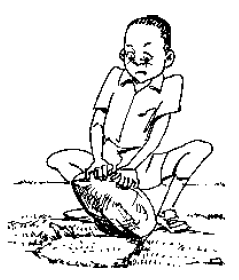
\includegraphics[width=0.35\textwidth]{./img/source/plants-light.png}
\end{center}

\begin{description*}
%\item[Subtopic:]{}
\item[Materials:]{Stone/brick or black plastic bag}
%\item[Setup:]{}
\item[Procedure:]{Cover an area of grass with a large flat brick/stone or with a black plastic bag so that no
light reaches the plants. Examine the grass after a few days. An alternative is to place a black
plastic bag over green leaves at the end of a branch and seal it by using string, tape or wire.}
%\item[Hazards:]{}
\item[Questions:]{What changes take place in the appearance of the leaves?}
\item[Observations:]{The plants and leaves become pale green or yellow in colour and die eventually.}
\item[Theory:]{Plants need light for photosynthesis. When they lose their green chlorophyll no more light
can be absorbed and they die.}
%\item[Applications:]{}
%\item[Notes:]{}
\end{description*}

\subsection{Extracting Chlorophyll} % Source 74

\begin{center}
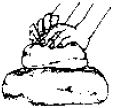
\includegraphics[width=0.25\textwidth]{./img/source/chlorophyll-extract.png}
\end{center}

\begin{description*}
%\item[Subtopic:]{}
\item[Materials:]{Green leaves, 2 rocks}
%\item[Setup:]{}
\item[Procedure:]{Pick about 5, large soft green leaves. Cut these into small pieces and grind with a stone.
Add a little water to the pulp and pour the mixture into a glass jar or test tune. Leave to settle.}
%\item[Hazards:]{}
%\item[Questions:]{}
\item[Observations:]{The solid material settles out, leaving a green solution.}
\item[Theory:]{The green substance in the water is chlorophyll, which has been released from the cells by
mechanical breaking of the cell membranes by grinding.}
%\item[Applications:]{}
\item[Notes:]{The extraction of chlorophyll works better in alcohol or spirit.}
\end{description*}

\subsection{Chlorophyll and Photosynthesis} % VSO 39, LASM 87

\begin{center}
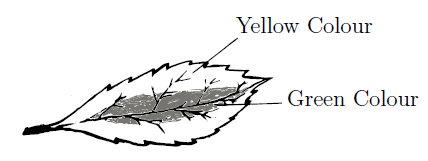
\includegraphics[width=0.4\textwidth]{./img/variegated-leaf.png}
\end{center}

\begin{description*}
%\item[Subtopic:]{}
\item[Materials:]{Variegated leaf, alcohol, water bath, \nameref{sec:heatsources}*, iodine solution}
%\item[Setup:]{}
\item[Procedure:]{Find a leaf which is not all green. Draw the
leaf, carefully identifying the
green areas where chlorophyll is
present. Test the leaf for starch.
(Boil the leaf in alcohol first).
}
%\item[Hazards:]{}
%\item[Questions:]{}
\item[Observations:]{The areas which turn
blue-black during the test are the
areas of the leaf which were
green.}
%\item[Theory:]{}
%\item[Applications:]{}
%\item[Notes:]{}
\end{description*}

\subsection{$\mathrm{CO_2}$ and Photosynthesis} % VSO 39, LASM 84

\begin{center}
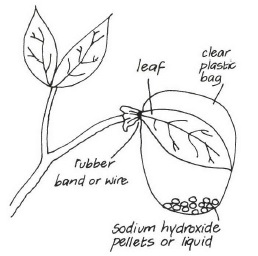
\includegraphics[width=0.35\textwidth]{./img/vso/co2-photo.jpg}
\end{center}

\begin{description*}
%\item[Subtopic:]{}
\item[Materials:]{Plant, clear plastic bag, rubber band/wire, sodium hydroxide, alcohol, water bath, \nameref{sec:heatsources}*, iodine solution}
%\item[Setup:]{}
\item[Procedure:]{Place a clear plastic bag over one
leaf of a plant as shown and leave
it for a day. Test the leaf in the
bag for starch and also test
another on the plant. (Boil leaves
in alcohol before testing for
starch.) }
%\item[Hazards:]{}
%\item[Questions:]{}
\item[Observations:]{The leaf which has been
in the bag will not have starch in
it, i.e. no photosynthesis has
taken place.}
\item[Theory:]{Sodium hydroxide absorbs carbon dioxide.}
%\item[Applications:]{}
%\item[Notes:]{}
\end{description*}

\subsection{Oxygen as a Product of Photosynthesis} % Source 74

\begin{center}
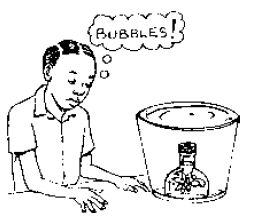
\includegraphics[width=0.4\textwidth]{./img/source/photo-gas.png}
\end{center}

\begin{description*}
%\item[Subtopic:]{}
\item[Materials:]{Plastic bottle, large container, water, plants}
%\item[Setup:]{}
\item[Procedure:]{Cut the neck from a plastic bottle, leaving the screw cap in place. Place in a large
container of water making sure the bottle is completely filled with water. Place some aquatic
plants under the bottle and leave for a few days in sunlight.}
%\item[Hazards:]{}
%\item[Questions:]{}
\item[Observations:]{The water level goes down. }
\item[Theory:]{Oxygen produced by photosynthesis forms as bubbles on the
leaves, which rise and collect in the bottle neck.}
%\item[Applications:]{}
%\item[Notes:]{}
\end{description*}

%\subsection{Oxygen as a By-Product of Photosynthesis} % LASM 91
%
%\begin{center}
%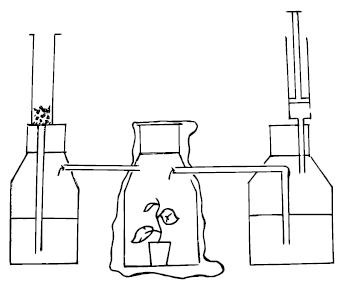
\includegraphics[width=0.4\textwidth]{./img/oxygen-photo.png}
%\end{center}
%
%\begin{description*}
%%\item[Subtopic:]{}
%\item[Materials:]{}
%\item[Setup:]{}
%\item[Procedure:]{}
%\item[Hazards:]{}
%\item[Questions:]{}
%\item[Observations:]{}
%\item[Theory:]{}
%\item[Applications:]{}
%\item[Notes:]{}
%\end{description*}

\subsection{Starch as a Product of Photosynthesis} % Source 75

\begin{center}
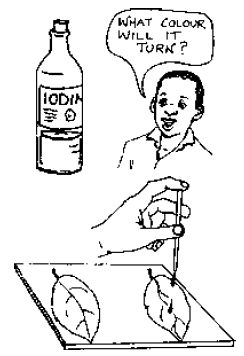
\includegraphics[width=0.4\textwidth]{./img/source/photo-starch.png}
\end{center}

\begin{description*}
%\item[Subtopic:]{}
\item[Materials:]{2 potted plants, alcohol, iodine solution, \nameref{sec:heatsources}*, straw}
%\item[Setup:]{}
\item[Procedure:]{Take two plants grown in pots and place one in sunlight and the other in a dark cupboard
for 2 days. Pick a leaf from each, but keep them separate. Heat each leaf in some alcohol for about 5 minutes to remove some of the green colour. Take each leaf out and lay it on
a flat surface. Add a few drops of iodine solution.}
%\item[Hazards:]{}
%\item[Questions:]{}
\item[Observations:]{The leaf from the plant grown in the light became a blue-black colour, whereas the one
from the dark was the pale brown colour of iodine.}
\item[Theory:]{When a leaf is exposed to light, photosynthesis occurs producing sugar, which is then
converted to starch for storage. This gives the blue/black colour with iodine. In the dark, no
photosynthesis can take place, so no starch is produced.}
%\item[Applications:]{}
%\item[Notes:]{}
\end{description*}

%\subsection{Light and Photosynthesis} % VSO 39
%
%\begin{center}
%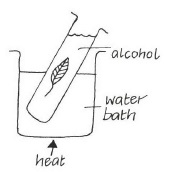
\includegraphics[width=0.4\textwidth]{./img/vso/photo-light.jpg}
%\end{center}
%
%\begin{description*}
%%\item[Subtopic:]{}
%\item[Materials:]{2 pot plants, dark cupboard, alcohol, \nameref{sec:heatsources}*, iodine solution}
%%\item[Setup:]{}
%\item[Procedure:]{Take 2 pot plants. Place one in
%sunlight and the other in a dark
%cupboard for 2-3 days. Pick a leaf
%from each plant and remove the
%green colour by heating the
%leaves for about 5 minutes in
%alcohol.
%Test each leaf for starch.}
%\item[Hazards:]{Do not heat the alcohol directly as it is a fire hazard.}
%%\item[Questions:]{}
%\item[Observations:]{The leaf receiving sunlight tests positive for starch, while the one in the cupboard does not.}
%%\item[Theory:]{}
%%\item[Applications:]{}
%%\item[Notes:]{}
%\end{description*}

%\subsection{Test for Starch in Leaves} % LASM 82 Move/combine above?
%
%\begin{center}
%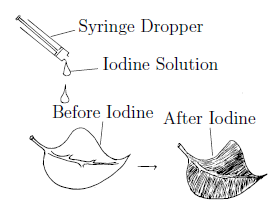
\includegraphics[width=0.4\textwidth]{./img/starch-leaf.png}
%\end{center}
%
%\begin{description*}
%%\item[Subtopic:]{}
%\item[Materials:]{}
%\item[Setup:]{}
%\item[Procedure:]{}
%\item[Hazards:]{}
%\item[Questions:]{}
%\item[Observations:]{}
%\item[Theory:]{}
%\item[Applications:]{}
%\item[Notes:]{}
%\end{description*}

%==================================================================================================%

%\section*{Food Preservation} 
%
%
%\subsection{Food Preservatives} % Bill Nye
%
%%\begin{center}
%%\includegraphics[width=0.4\textwidth]{./img/.png}
%%\end{center}
%
%\begin{description*}
%%\item[Subtopic:]{}
%\item[Materials:]{}
%\item[Setup:]{}
%\item[Procedure:]{}
%\item[Hazards:]{}
%\item[Questions:]{}
%\item[Observations:]{}
%\item[Theory:]{}
%\item[Applications:]{}
%\item[Notes:]{}
%\end{description*}

%==================================================================================================%


\end{multicols}

\pagebreak